\documentclass[10pt]{beamer}%
 \usetheme[progressbar = foot, background=light, numbering=none]{metropolis} 
 %\usecolortheme[cautious]{owl} %owl-defined colours will be available as OwlRed, OwlGreen, and so forth.
 \setbeamercolor{title separator}{fg=OwlGreen}
%\setsansfont{Ubuntu}
%\setmonofont{Ubuntu Mono}
% % input
% 
\useoutertheme{split}
%\setbeamertemplate{footline}{\small \insertauthor}

\usepackage[utf8]{inputenc}%
 \usepackage{lmodern} %Type1-font for non-english texts and characters
 \usepackage[USenglish]{babel} %francais, polish, spanish, ...
 \usepackage[T1]{fontenc}
% 
 \usepackage{ragged2e}%for text justification by default
 \justifying
% 
 % graphics
 %% Figures %%%%%%%%%%%%%%%%%%%%%%%%%%%%%%%%%%%%%%%%%%%%%%%%%%
 \usepackage{graphicx}
 
 \hypersetup{pdfstartview={Fit}} % fits the presentation to the window when first displayed
 
 \title[]{}
 \date{March 22, 2017}
 \author[\footnotesize Timoth\'ee Bonnet ]{ }

%%%%%%%%%%%%%%%%%%%%%%%%%%%%%%%%%%%%%%%%%%%%%%
\begin{document}

\begin{frame}{Timoth\'ee Bonnet}

\vfill

\includegraphics[width=0.03\textwidth]{Figures/tweeter.jpeg} @TimotheeBonnet
\end{frame}
%%%%%%%%%%%
\begin{frame}{Evolutionary quantitative genetics}
   
    \begin{alertblock}{How fast are wild vertebrates evolving?}
        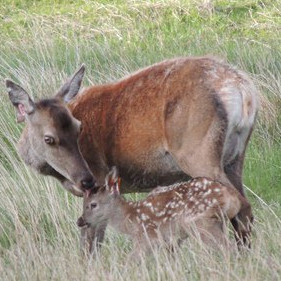
\includegraphics[width=0.15\textwidth]{Figures/doe}
        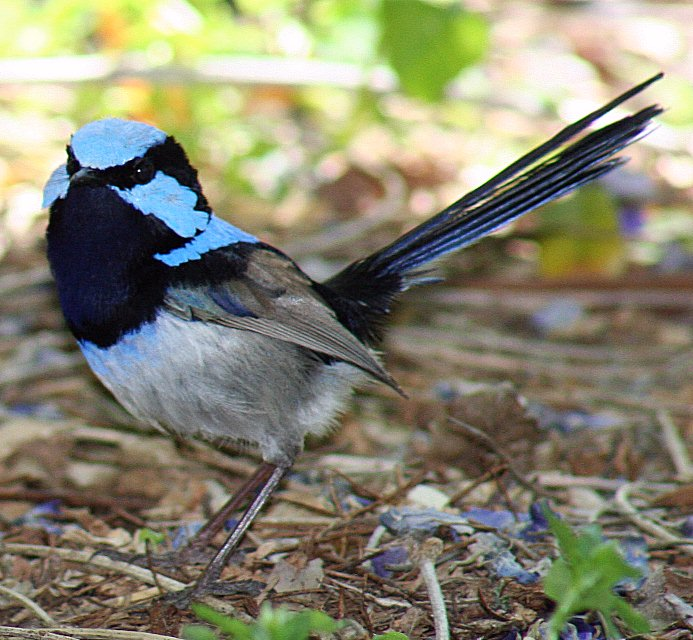
\includegraphics[width=0.15\textwidth]{Figures/sfw}
        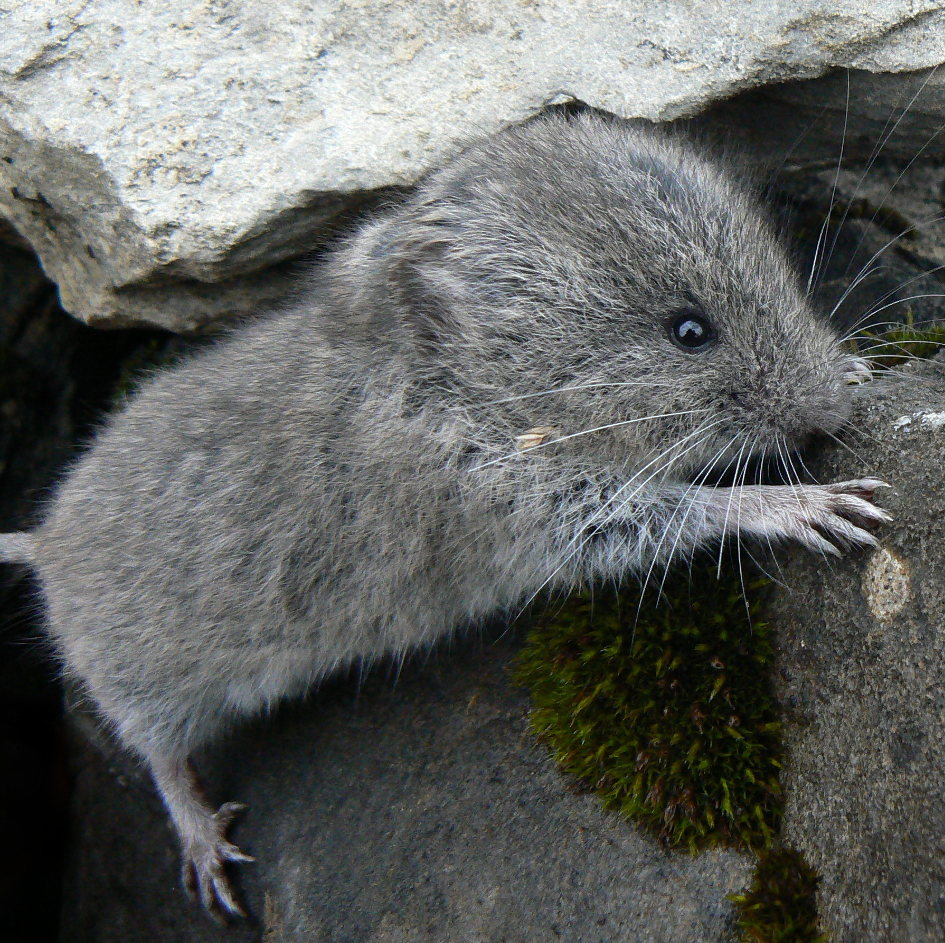
\includegraphics[width=0.15\textwidth]{Figures/vole}
        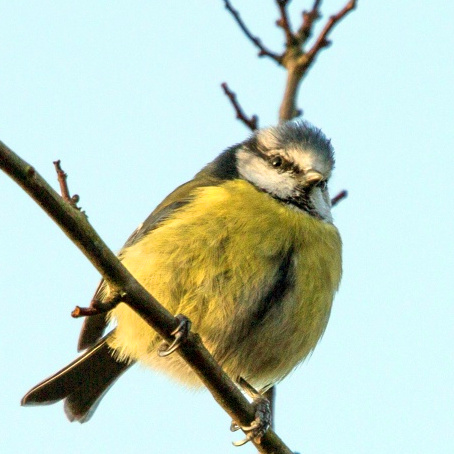
\includegraphics[width=0.15\textwidth]{Figures/bt}
        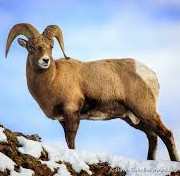
\includegraphics[width=0.15\textwidth]{Figures/bgs}
        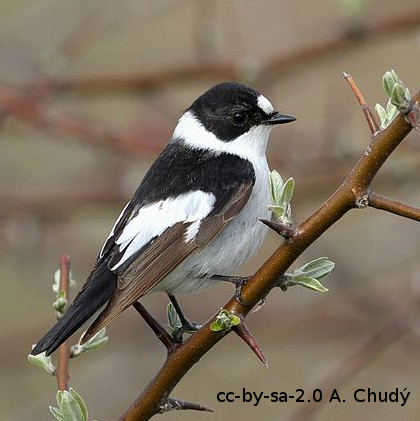
\includegraphics[width=0.15\textwidth]{Figures/cfc}
    \end{alertblock}

\end{frame}
%%%%%%%%%%%
%%%%%%%%%%%
\begin{frame}{Statistics, coding}

\end{frame}
%%%%%%%%%%%
%%%%%%%%%%%
\begin{frame}{Naturalism}

\end{frame}
%%%%%%%%%%%

\end{document}
